\chapter{DI, TPI, y el fenómeno actual que me está sucediendo}

	\noindent
	Ambas, la DI y la TPI, son ``juegos cardinales''. La DI es más vieja y es menos ``rigurosa'' en su exposición. Las dos parten del supuesto, que si el conjunto que hace el papel de Dominio, es ABSURDAMENTE mucho mayor que el otro, si su diferencia cardinal es INCONMENSURABLE, :D, no deberían poder construirse con éxito. Y si se construyen con éxito, ambas implican que el cardinal del Dominio, NO es mayor que el cardinal del otro conjunto (que no tiene porque ser el conjunto Imagen, ojo). Lo cual implica que pueden ser iguales.

	\section{DI:variante pelea de colegio}
	
	\noindent
	DI significa Diagonalización Inversa. Busca un fenómeno similar a la diagonalización, invirtiendo los papeles conocidos de las cardinalidades $\aleph_{1}$ y $\aleph_{0}$. Da igual que barras todas las opciones disponibles para el Dominio ($\aleph_{1}$), NUNCA podrá 'cubrir´ todos los elementos del conjunto con cardinalidad $\aleph_{0}$.
	\\\\
	
	\noindent
	Consiste en que dos alumnos de un colegio se quieren pelear, comparando la cantidad de amigos que cada uno puede aportar a la pelea. Los amigos de Domenicus (Dominio: D) y los amigos de Luciferio\footnote{Lucifer: portador de Luz, Luz $\rightarrow$ Imagen :D.} (Imagen: I). Domenicus le ha dicho a Luciferio que las paradojas híbridas no existen, y no le deja a Luciferio reproducir el experimento que así lo demuestra\footnote{Déjame descargar frustración en alguna parte...}. Antes de que esta afrenta al honor acabe en un baño de sangre, Luciferio le dice a Domenicus que más le vale rendirse ya que tiene amigos suficientes como para estar en una proporción 2 a 1 o superior.
	\\\\
	
	\noindent
	Domenicus no se fía de Luciferio, tiene fama de tramposo, así que le exige una lista detallada que diga, exactamente, que amigos suyos se van a pelear con cada uno de sus amigos. Así que Luciferio le entrega este esquema (Empecemos por un caso finito, para entender el juego):
	\\\\
	
	\noindent
	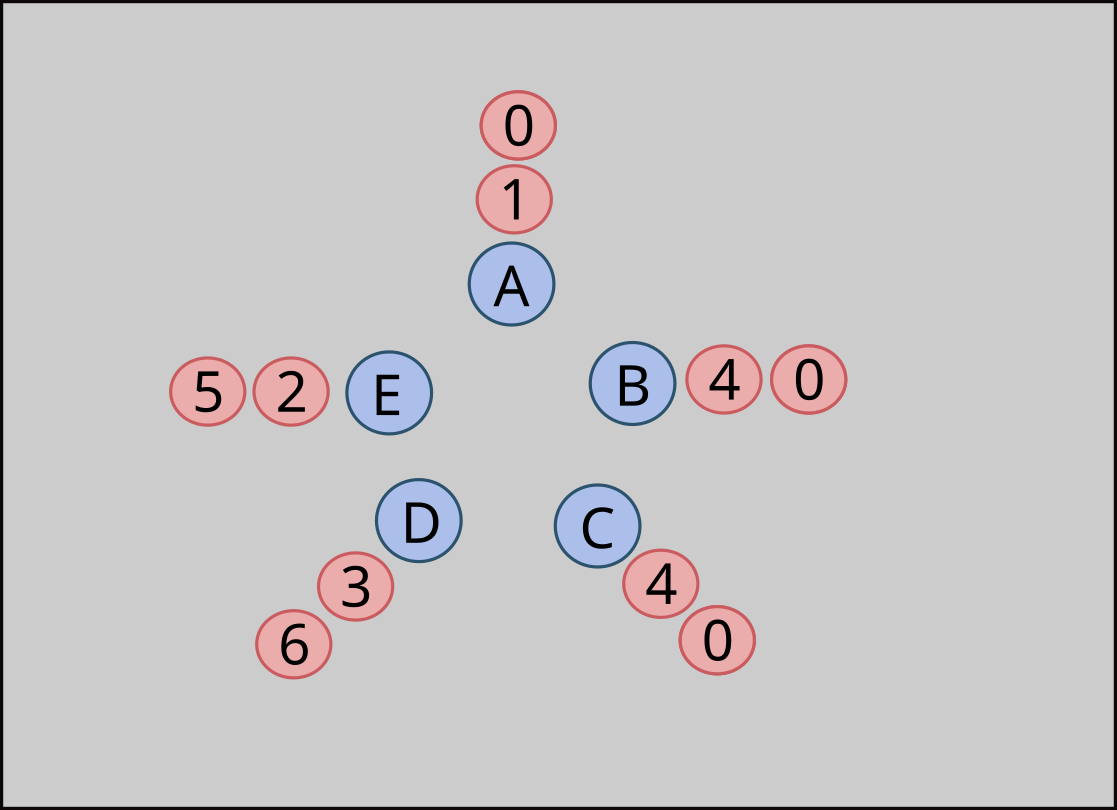
\includegraphics[scale=0.5]{Distribucion_001_A}\\\\
	Como en este colegio son gente muy rara, los amigos de Domenicus tienen nombre de letra, y los de Luciferio tienen nombre de número natural. Vemos que cada amigo de Domenicus(D) tiene un ``Pack'' de amigos de Luciferio(I) asignados. El cardinal de esos Packs es de 2... así que aparentemente Luciferio no mentía con su amenaza.
	\\\\
	
	\noindent
	Después de observar un rato, Domenicus se da cuenta que Luciferio ha hecho trampas: ha puesto a su amigo ``$0$'', dentro del Pack de dos de sus amigos: A y B. Se queja a Luciferio, y este le dice: ``¿Sabes qué, quita a $0$ de la pelea, lo retiro, y si encuentras más repeticiones de uso, también los retiraré de la pelea''. Domenicus luego se fija en que $0$ también está dentro del Pack de C. Luciferio le dice que cuando apartas a uno de sus amigos de la pelea, eso significa quitarlo de TODOS los Packs donde pudiese estar. Así lo hacen y el esquema queda así:\\\\
	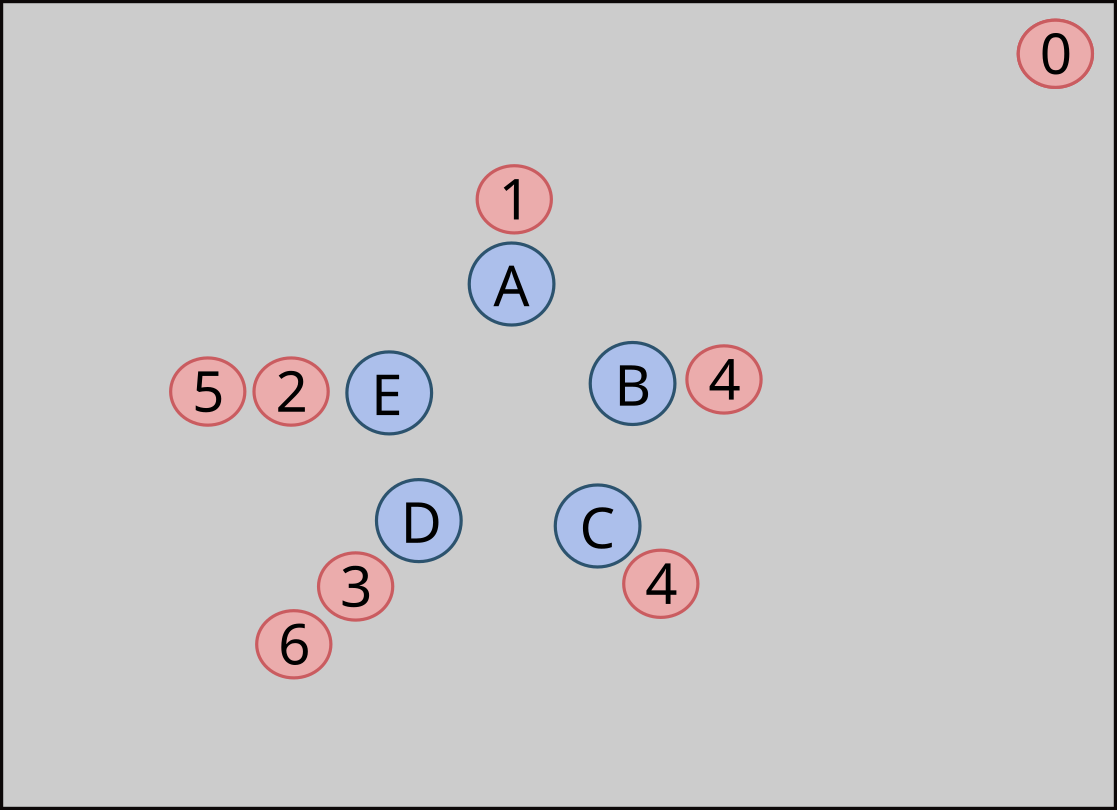
\includegraphics[scale=0.5]{Distribucion_001_B}
	\\\\
	
	\noindent
	Domenicus, que es conocedor de técnicas secretas y avanzadas en teoría de conjuntos, sigue buscando par por par, para ver si Luciferio ha hecho más trampas o si efectivamente, después de descartar a $0$, los Packs nuevos creados a partir del primer esquema (la relación no aplicación original), cumplen las condiciones del Naive CA Theorem.
	\\\\
	
	\noindent
	Domenicus pregunta por el actual estado de los pares (E,D), (D,C), (E,A)... (A,B). Los nuevos Packs de (A,B) son más pequeños que los originales, pero ahora son disjuntos, así que este par no da más problemas. Y cuando se empieza a desesperar, Domenicus encuentra el par (B,C). Tienen el 4 repetido. Siguiendo el acuerdo con Luciferio, 4 se retira de la pelea y lo ``retiran'' de todos los Packs donde pudiese estar:
	\\\\
	
	\noindent
	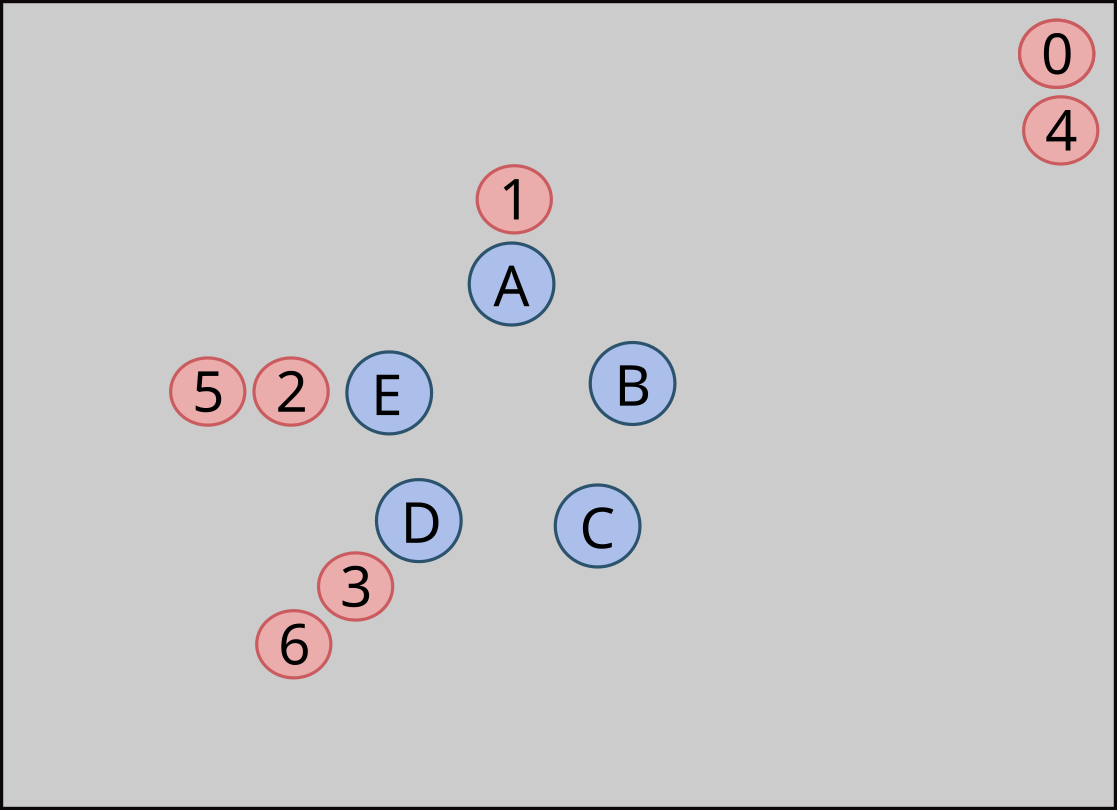
\includegraphics[scale=0.45]{Distribucion_001_C}
	\\\\
	
	\noindent
	Ahora, B y C, tienen Packs asignados completamente vacíos. Domenicus se ríe de Luciferio:``No solo mentiste con la proporción 2 a 1, sino que ni siquiera cumples el Naive CA theorem!!''. Luciferio se enfada mucho, llama a más amigos e intenta otra distribución nueva:
	\\\\
	
	\noindent
	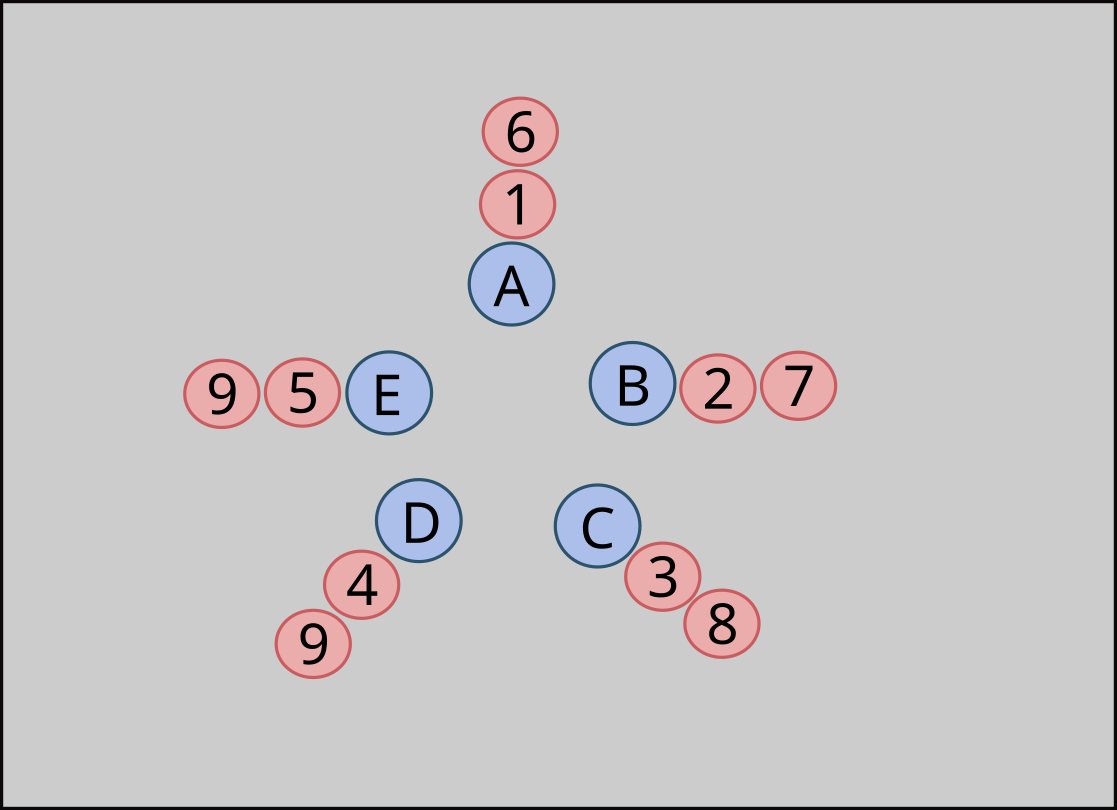
\includegraphics[scale=0.45]{Distribucion_002_A}
	\\\\
	
	\newpage
	
	
	
	
	
	
	
	\section{TPI}
	
	
	
	\section{Resultado increíble}